\section{Experimental Results}

\subsection*{Evaluation Metrics}
We use two metrics to measure model accuracy, using the cardiologist committee
annotations as the ground truth.

\textbf{Sequence Level Accuracy (F1):} We measure the average overlap between
the prediction and the ground truth sequence labels. For every record, a model
is required to make a prediction approximately once per second (every 256
samples). These predictions are compared against the ground truth annotation.

\textbf{Set Level Accuracy (F1):} Instead of treating the labels for a record
as a sequence, we consider the set of unique arrhythmias present in each 30
second record as the ground truth annotation. Set Level Accuracy, unlike
Sequence Level Accuracy, does not penalize for time-misalignment within a
record. We report the F1 score between the unique class labels from the ground
truth and those from the model prediction.

In both the Sequence and the Set case, we compute the F1 score for each class
separately. We then compute the overall F1 (and precision and recall) as the
class-frequency weighted mean.

\subsection*{Model vs. Cardiologist Performance} We assess the cardiologist
performance on the test set. Recall that each of the records in the test set
has a ground truth label from a committee of three cardiologists as well as
individual labels from a disjoint set of 6 other cardiologists. To assess
cardiologist performance for each class, we take the average of all the
individual cardiologist F1 scores using the group label as the ground truth
annotation.

Table~\ref{tab:HumanVsModel} shows the breakdown of both cardiologist and model
scores across the different rhythm classes. The model outperforms the average
cardiologist performance on most rhythms, noticeably outperforming the
cardiologists in the AV Block set of arrhythmias which includes Mobitz I
(Wenckebach), Mobitz II (AVB\_Type2) and complete heart block (CHB). This is
especially useful given the severity of Mobitz II and complete heart block and
the importance of distinguishing these two from Wenckebach which is usually
considered benign.

Table~\ref{tab:HumanVsModel} also compares the aggregate precision, recall and
F1 for both  model and cardiologist compared to the ground truth annotations.
The aggregate scores for the cardiologist are computed by taking the mean of
the individual cardiologist scores. The model outperforms the cardiologist
average in both precision and recall.

\begin{figure}
\centering
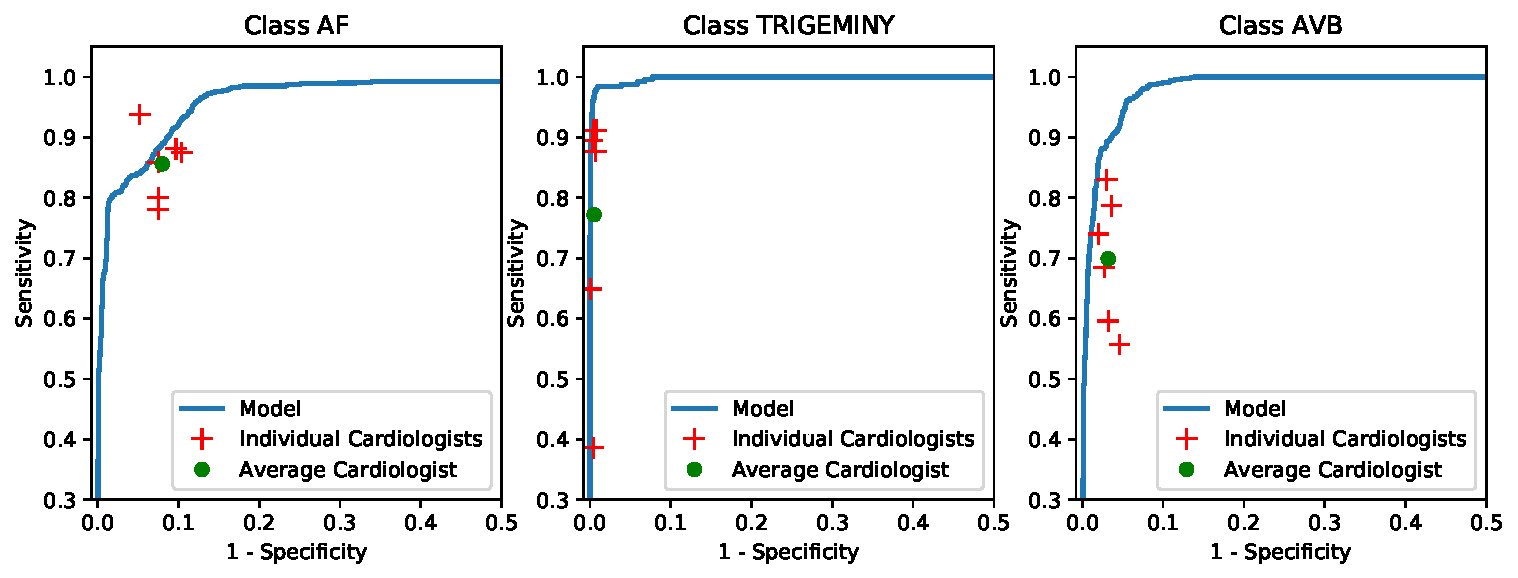
\includegraphics[width=1.0\textwidth]{arrhythmias/figures/roc_curve.pdf}
\caption{Receiver operating characteristic curves at sequence-level for atrial
         fibrillation (AF), trigeminy and atrioventricular block (AVB).}
\label{fig:arrhythmias:roc_curve}
\end{figure}

\begin{figure}
\centering
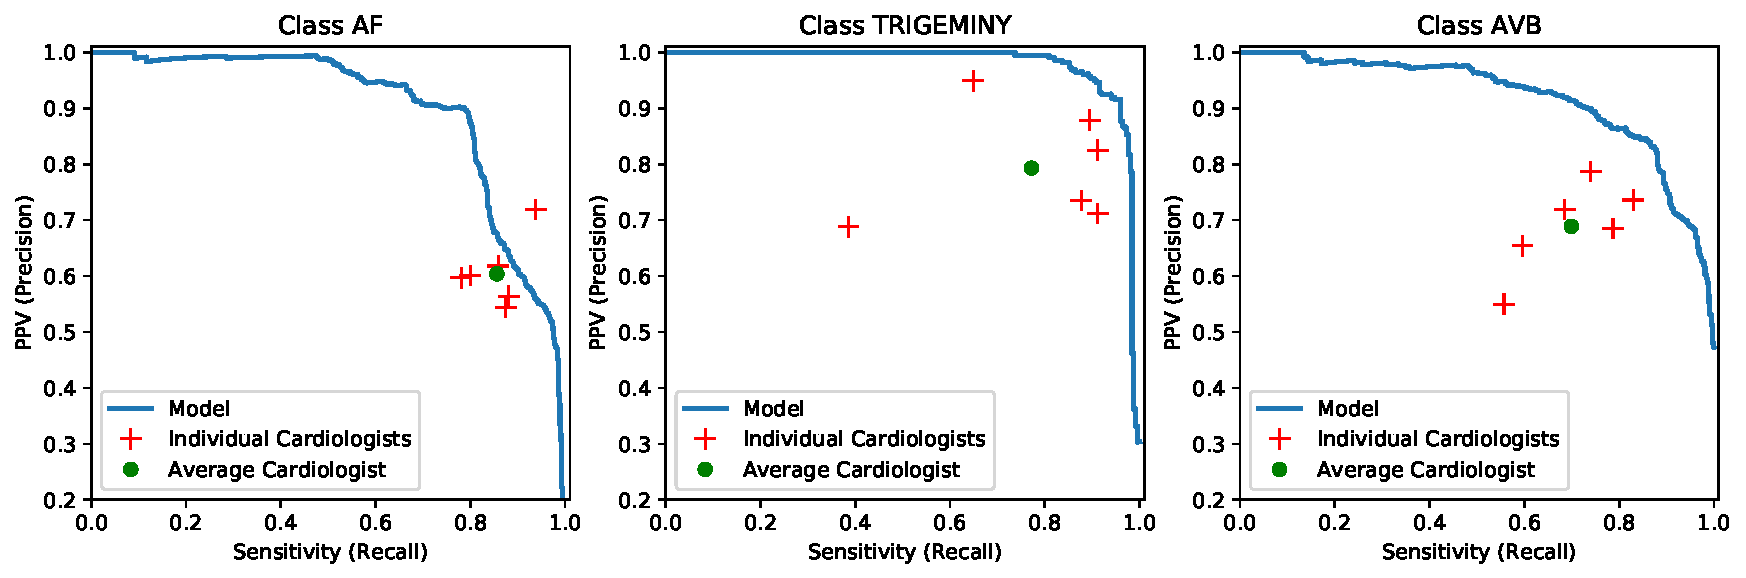
\includegraphics[width=1.0\textwidth]{arrhythmias/figures/prec_recall_curve.pdf}
\caption{Precision-Recall curves at sequence-level for atrial fibrillation,
         trigeminy and atrioventricular block.}
\label{fig:arrhythmias:prec_recall_curve}
\end{figure}
